\subsection{Kommunikation zwischen Freedom-Board und Android-Phone}
\begin{tabular}{p{4.5cm}p{\textwidth-3.6cm-0.7cm}}
    \rule{0pt}{11pt}\textit{Tester}              & Thomas Wiss \\ 
    \rule{0pt}{11pt}\textit{Datum}:           & 16.04.2015   \\
    \rule{0pt}{11pt}\textit{Ort}:             & Teaminsel \\
    \rule{0pt}{11pt}\textit{Beschreibung}:          & Um den auf dem Android-Phone berechneten 
    Winkel zum Freedom-Board zu senden, muss die Kommunikation zwischen dem Freedom-Board 
    und dem Android-Phone getestet werden. \\
    \rule{0pt}{11pt}\textit{Akteure}:          & Operator zur Bedienung des Android-Phones. \\
    \rule{0pt}{11pt}\textit{Bedingung}:          & USB-Kabel muss am Android-Phone und gleichzeitig 
    auch am Freedom-Board eingesteckt sein. \\
    \rule{0pt}{11pt}\textit{Erwartete Fehlermeldung}:          & keine \\
    \rule{0pt}{11pt}\textit{Vorgehen}:          & USB-Kabel am Android-Phone und am 
    Freedom-Board einstecken. Starten der Applikation \enquote{SerialPortExample} auf dem Android-Phone. 
    Den Befehl \enquote{debug} ins Textfeld eintragen und den Button Send betätigen. \\
    \rule{0pt}{11pt}\textit{Erwartetes Ergebnis}:          & Die Rückmeldung in der TextBox 
    muss ein Informations- und Hilfemenu anzeigen. \\
    \rule{0pt}{11pt}\textit{Eingetretenes Ergebnis}:          & Siehe Abbildung 
    \ref{abb:ScreenshotSerialPortExampleTestProtokol}. \\
    \rule{0pt}{11pt}\textit{Test bestanden?}:          & Ja \\
    \rule{0pt}{11pt}\textit{Weiter Tests nötig?}:          & Nein \\
\end{tabular}    
    \newline
    \newline
    \begin{figure}[h!]
    	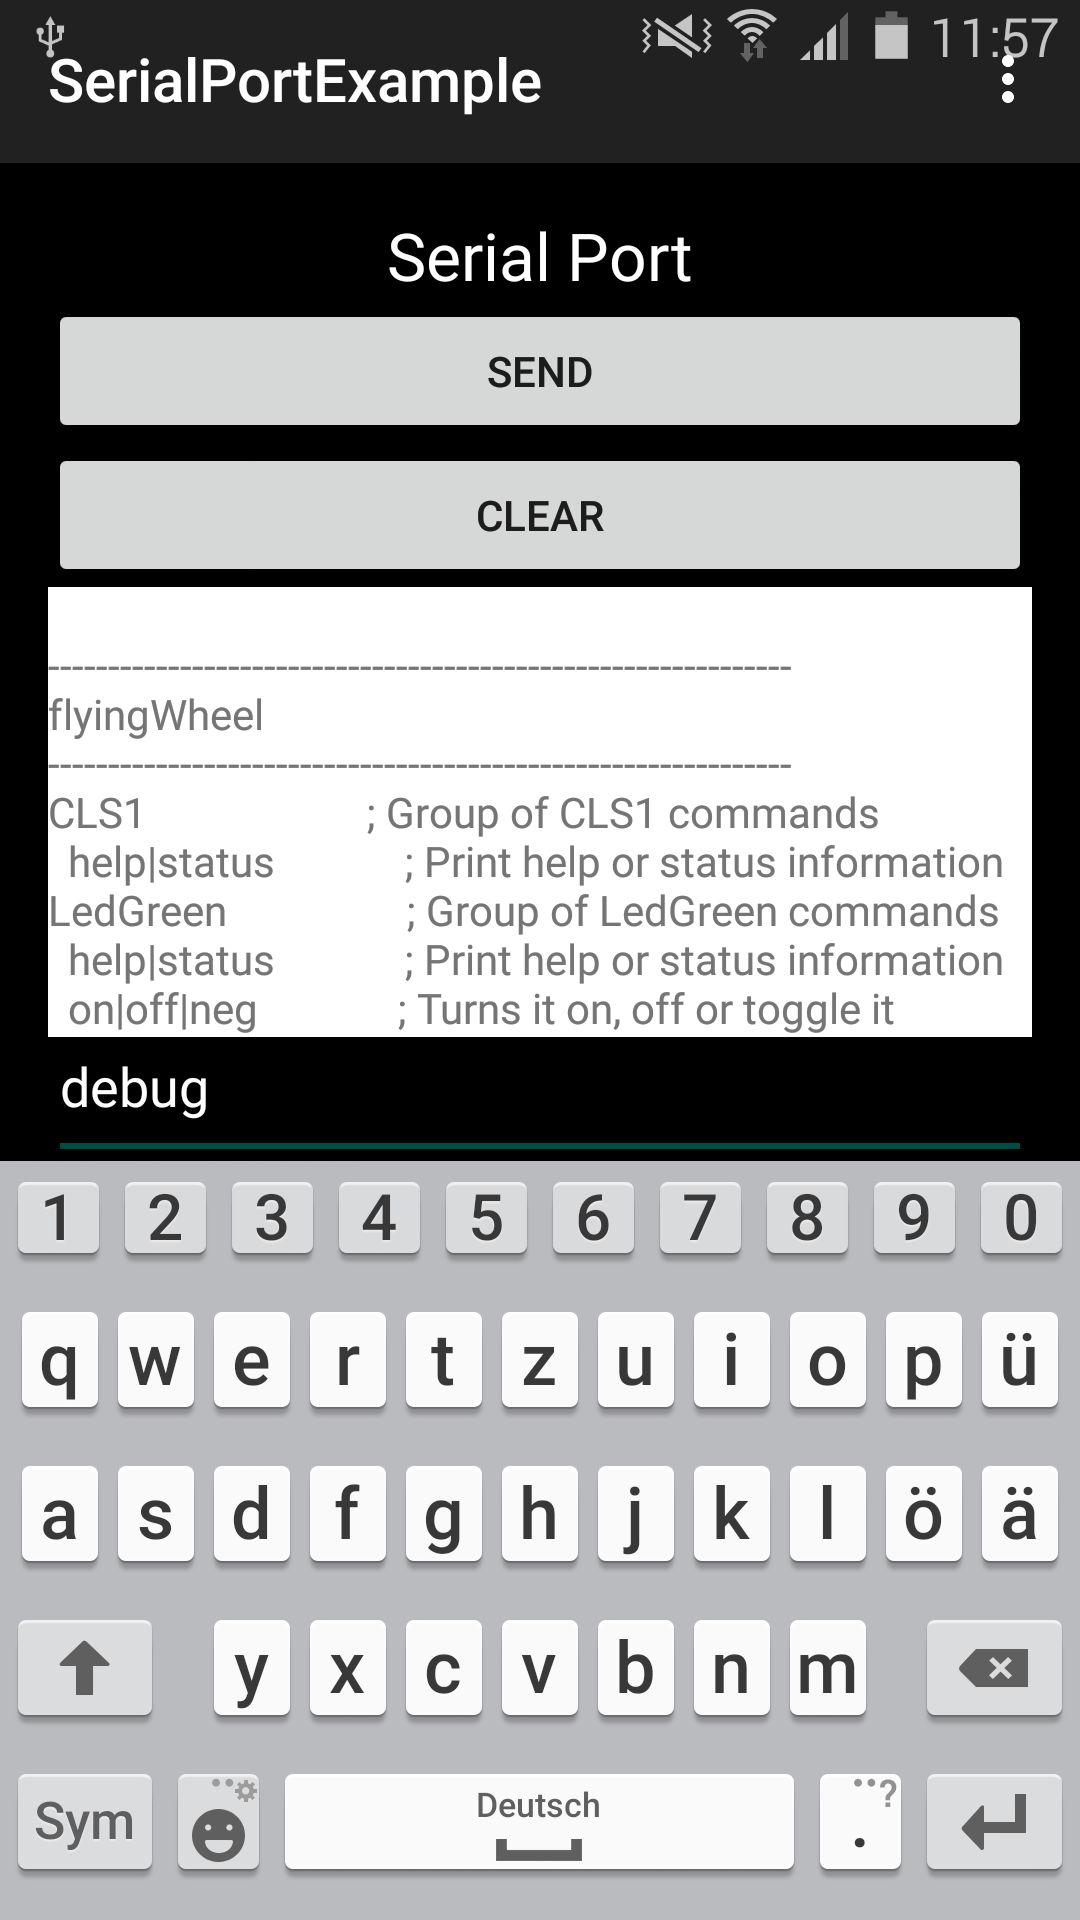
\includegraphics[width=0.3\textwidth,clip,trim=0mm 0mm 0mm 0mm]
    	{Enddokumentation/Bilder/Screenshot_SerialPortExample_debug.png}
    	\centering
    	\caption{Screenshot der Applikation \enquote{SerialPortExample}}
    	\label{abb:ScreenshotSerialPortExampleTestProtokol}
    \end{figure}
    
